\documentclass[aspectratio=169,10pt]{beamer}

% ============================================================
%  PAQUETES
% ============================================================
\usepackage[T1]{fontenc}
\usepackage[utf8]{inputenc}
\usepackage{amsmath,amssymb,bm}
\usepackage{tikz}
\usetikzlibrary{arrows.meta,positioning,calc,backgrounds,shapes.geometric}
\usepackage{tcolorbox}
\tcbuselibrary{skins,breakable}
\usepackage{booktabs}
\usepackage{xcolor}
\usepackage{listings}

% ============================================================
%  PALETA
% ============================================================
\definecolor{darkbg}{HTML}{1A1A2E}
\definecolor{accent}{HTML}{E94560}
\definecolor{accentteal}{HTML}{0F9B8E}
\definecolor{accentamber}{HTML}{F5A623}
\definecolor{accentviolet}{HTML}{7B68EE}
\definecolor{textlight}{HTML}{EAEAEA}
\definecolor{textgray}{HTML}{9E9E9E}
\definecolor{lightbg}{HTML}{F7F7F7}
\definecolor{coralbox}{HTML}{FF6B6B}

% ============================================================
%  TEMA BEAMER
% ============================================================
\setbeamercolor{background canvas}{bg=lightbg}
\setbeamercolor{normal text}{fg=darkbg}
\setbeamertemplate{navigation symbols}{}
\setbeamertemplate{footline}{%
  \hfill\textcolor{textgray}{\tiny\texttt{mbastidaso@unal.edu.co}%
  \quad\insertframenumber/\inserttotalframenumber\quad}%
  \vspace{4pt}%
}
\setbeamertemplate{itemize item}{\textcolor{accent}{\textbullet}}
\setbeamertemplate{itemize subitem}{\textcolor{accentteal}{--}}

% ============================================================
%  ENTORNO DARK SLIDE
% ============================================================
\newenvironment{darkslide}{%
  \setbeamercolor{background canvas}{bg=darkbg}%
  \setbeamercolor{normal text}{fg=textlight}%
}{%
  \setbeamercolor{background canvas}{bg=lightbg}%
  \setbeamercolor{normal text}{fg=darkbg}%
}

% ============================================================
%  CAJAS DE CONTENIDO
% ============================================================
\tcbset{mybase/.style={
  enhanced, breakable, arc=3pt,
  boxrule=0.6pt, left=6pt, right=6pt, top=5pt, bottom=5pt,
  fonttitle=\small\bfseries, fontupper=\small
}}
\newtcolorbox{defbox}[1]{mybase,
  colback=accentviolet!8, colframe=accentviolet!60, title={#1}}
\newtcolorbox{resultbox}[1]{mybase,
  colback=accentteal!8, colframe=accentteal!60, title={#1}}
\newtcolorbox{obsbox}[1]{mybase,
  colback=accentamber!10, colframe=accentamber!70, title={#1}}
\newtcolorbox{taskbox}[1]{mybase,
  colback=coralbox!8, colframe=coralbox!60, title={#1}}

\newcommand{\R}{\mathbb{R}}

% ============================================================
\begin{document}
% ============================================================

% ── PORTADA ──────────────────────────────────────────────────
\begin{darkslide}
\begin{frame}[plain]
\begin{tikzpicture}[remember picture, overlay]
  \fill[accent,opacity=0.15]      (current page.north east) ++(-1.5,-1.5) circle (4cm);
  \fill[accentteal,opacity=0.10]  (current page.south west) ++(2,2)       circle (3cm);
  \fill[accentviolet,opacity=0.08](current page.north west) ++(1,-2)       circle (2.5cm);
\end{tikzpicture}
\vspace{1.5cm}
\begin{center}
  {\small\textcolor{textgray}{Programaci\'on Cient\'ifica $\cdot$ 2026-1}}\\[16pt]
  {\LARGE\textcolor{textlight}{\textbf{Sistemas Din\'amicos}}}\\[6pt]
  {\large\textcolor{accent}{M\'odulo 4 - Clase 1}}\\[14pt]
  {\normalsize\textcolor{textgray}{%
    ?`Puede una ecuaci\'on describir c\'omo cambia una sociedad?}}\\[20pt]
  {\normalsize\textcolor{textgray}{Universidad Nacional de Colombia}}\\[4pt]
  {\small\textcolor{textgray}{\texttt{mbastidaso@unal.edu.co}}}
\end{center}
\end{frame}
\end{darkslide}


% ── SECCIÓN: ¿QUÉ ES UN SISTEMA DINÁMICO? ───────────────
\begin{darkslide}
\begin{frame}[plain]
\begin{tikzpicture}[remember picture, overlay]
  \fill[accentteal,opacity=0.12](current page.south east)++(-2,2)  circle(3.5cm);
  \fill[accent,opacity=0.08]    (current page.north west)++(2,-1)  circle(2.5cm);
\end{tikzpicture}
\vspace{2.5cm}
\begin{center}
  {\LARGE\textcolor{textlight}{\textbf{%
    ?`Qu\'e es un sistema din\'amico?}}}
\end{center}
\end{frame}
\end{darkslide}

% ─────────────────────────────────────────────────────────
\begin{frame}{Estado y espacio de estados}
\begin{columns}[T]
\column{0.50\textwidth}
\begin{defbox}{Estado}
El \textbf{estado} $x(t)$ es toda la informaci\'on del sistema en el instante $t$
que determina su evoluci\'on futura.
\end{defbox}

\vspace{8pt}
\textbf{Ejemplos:}
\begin{itemize}\small
  \item Opini\'on de $N$ personas:\quad
        $x = (x_1,\ldots,x_N)\in\R^N$.
  \item Fase de $N$ osciladores:\quad
        $\theta = (\theta_1,\ldots,\theta_N)\in\R^N$.
  \item Temperatura de un s\'olido:\quad
        $T \in \R^+$.
\end{itemize}

\vspace{6pt}
El conjunto de todos los estados posibles es el
\textbf{espacio de estados} $\mathcal{X}$.

\column{0.46\textwidth}
\begin{defbox}{Trayectoria}
La \textbf{trayectoria} $x:\R\to\mathcal{X}$ es la curva
que recorre el estado a lo largo del tiempo.
\end{defbox}

\vspace{6pt}
\begin{center}
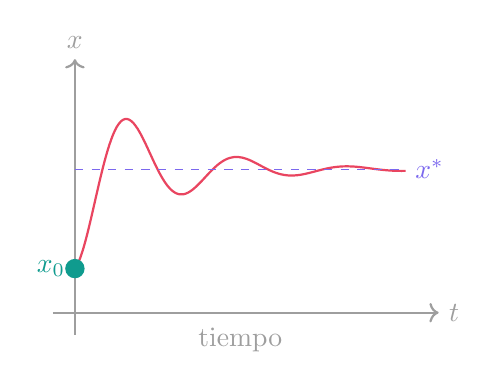
\begin{tikzpicture}[scale=1.4]
  \draw[->,thick,textgray](-0.2,0)--(3.3,0)node[right]{$t$};
  \draw[->,thick,textgray](0,-0.2)--(0,2.3)node[above]{$x$};
  % trayectoria amortiguada
  \draw[accent,thick,smooth]
    plot[variable=\t,domain=0:3,samples=80]
    ({\t},{1.3-0.9*exp(-1.4*\t)*cos(360*\t)});
  % punto inicial
  \fill[accentteal](0,0.4)circle(2.5pt)node[left]{$x_0$};
  % punto de equilibrio
  \draw[accentviolet,dashed,thin](0,1.3)--(3,1.3)
        node[right]{$x^*$};
  \node[below=2pt,font=\color{textgray}] at (1.5,0){tiempo};
\end{tikzpicture}
\end{center}
\end{columns}
\end{frame}

% ─────────────────────────────────────────────────────────
\begin{frame}{La EDO como lenguaje}
\vspace{4pt}
\begin{defbox}{Ecuaci\'on diferencial ordinaria (EDO)}
\[
  \dot{x}(t) = f\!\bigl(x(t),\,t\bigr), \qquad x(t_0) = x_0
\]
\begin{itemize}
  \item $f:\mathcal{X}\times\R\to\mathcal{X}$  \textbf{campo vectorial}:
        especifica direcci\'on y velocidad de cambio.
  \item La EDO no dice \emph{d\'onde est\'a} $x$; dice \emph{c\'omo cambia}.
  \item $x_0$  \textbf{condici\'on inicial}: fija la trayectoria.
\end{itemize}
\end{defbox}

\vspace{8pt}
\begin{resultbox}{Teorema de Picard-Lindel\"of (enunciado informal)}
Si $f$ es continua y (local) Lipschitz en $x$, existe una \'unica soluci\'on
$x(t)$ en un intervalo $[t_0,\,t_0+\delta)$.\\[3pt]
\textcolor{textgray}{\small
El modelo est\'a bien planteado: dado $x_0$, la trayectoria queda determinada.}
\end{resultbox}
\end{frame}

% ─────────────────────────────────────────────────────────
\begin{frame}{Tipos de sistemas din\'amicos}
\vspace{4pt}
\begin{center}
\renewcommand{\arraystretch}{1.45}
\begin{tabular}{lll}
\toprule
\textbf{Eje} & \textbf{Opci\'on A} & \textbf{Opci\'on B} \\
\midrule
Tiempo       & Discreto ($t\in\mathbb{Z}$,\; $x_{n+1}=g(x_n)$)
             & Continuo ($t\in\R$,\; EDO $\dot{x}=f(x,t)$) \\
Autonom\'ia  & No aut\'onomo:\; $f=f(x,t)$
             & Aut\'onomo:\; $f=f(x)$ \\
Linealidad   & Lineal:\; $f(x)=Ax$
             & No lineal:\; $f$ arbitraria \\
Incertidumbre& Determinista
             & Estoc\'astico \\
\bottomrule
\end{tabular}
\end{center}

\vspace{10pt}
\begin{obsbox}{Los modelos de este m\'odulo}
\textbf{Hegselmann-Krause}: continuo, aut\'onomo, \textbf{no lineal}.\\[3pt]
\textbf{Kuramoto}: continuo, aut\'onomo, \textbf{no lineal}. \\[3pt]
Ambos son deterministas: dada $x_0$, la trayectoria es \'unica.
\end{obsbox}
\end{frame}

% ── SECCIÓN: CICLO DE MODELACIÓN ─────────────────────────
\begin{darkslide}
\begin{frame}[plain]
\begin{tikzpicture}[remember picture, overlay]
  \fill[accentamber,opacity=0.12](current page.north west)++(2,-2) circle(3cm);
  \fill[accentteal,opacity=0.08] (current page.south east)++(-2,2) circle(3cm);
\end{tikzpicture}
\vspace{2.5cm}
\begin{center}
  {\LARGE\textcolor{textlight}{\textbf{El ciclo de modelaci\'on}}}
\end{center}
\end{frame}
\end{darkslide}

% ─────────────────────────────────────────────────────────
\begin{frame}{Del fen\'omeno a la ecuaci\'on}
\vspace{2pt}
\begin{center}
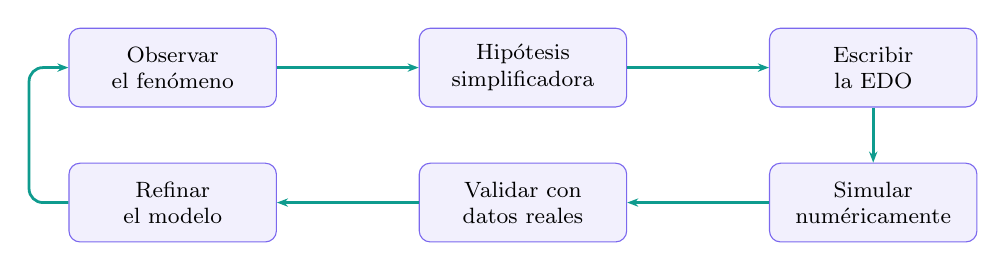
\begin{tikzpicture}[
  node distance=7mm and 18mm,
  box/.style={rounded corners=4pt,draw=accentviolet,fill=accentviolet!10,
              minimum width=26mm,minimum height=10mm,
              font=\footnotesize,align=center,text width=24mm},
  arr/.style={-{Stealth[length=4pt]},accentteal,line width=1pt}
]
  \node[box](obs){Observar\\el fen\'omeno};
  \node[box,right=of obs](hip){Hip\'otesis\\simplificadora};
  \node[box,right=of hip](eq){Escribir\\la EDO};
  \node[box,below=of eq](sim){Simular\\num\'ericamente};
  \node[box,left=of sim](val){Validar con\\datos reales};
  \node[box,left=of val](ref){Refinar\\el modelo};

  \draw[arr](obs)--(hip);
  \draw[arr](hip)--(eq);
  \draw[arr](eq) --(sim);
  \draw[arr](sim)--(val);
  \draw[arr](val)--(ref);
  \draw[arr,rounded corners=5pt](ref.west)--++(-5mm,0)
       |-(obs.west);
\end{tikzpicture}
\end{center}

\vspace{6pt}
\begin{obsbox}{Esta clase}
Seguiremos este ciclo en vivo para construir el modelo H-K.\\
Empezamos con la \textbf{observaci\'on}: ?`por qu\'e las redes sociales
nos polarizan?
\end{obsbox}
\end{frame}

% ── SECCIÓN: MODELO H-K ───────────────────────────────────
\begin{darkslide}
\begin{frame}[plain]
\begin{tikzpicture}[remember picture, overlay]
  \fill[coralbox,opacity=0.12]    (current page.north east)++(-2,-2) circle(3.5cm);
  \fill[accentviolet,opacity=0.10](current page.south west)++(1,1)   circle(3cm);
\end{tikzpicture}
\vspace{2cm}
\begin{center}
  {\Large\textcolor{textlight}{\textbf{Construcci\'on}}}\\[10pt]
  {\large\textcolor{coralbox}{Modelo de Hegselmann-Krause}}\\[6pt]
  {\normalsize\textcolor{textgray}{?`Por qu\'e internet nos polariza?}}
\end{center}
\end{frame}
\end{darkslide}

% ─────────────────────────────────────────────────────────
\begin{frame}{Observaci\'on: el l\'imite de confianza}
\vspace{4pt}
\begin{taskbox}{Pausa}
?`Qu\'e hace que tu opini\'on cambie?\\[4pt]
?`Qu\'e hace que ignores completamente la opini\'on de alguien?
\end{taskbox}

\vspace{10pt}
\textbf{Hip\'otesis (Hegselmann \& Krause, 2002):}
\begin{itemize}
  \item Cada individuo tiene una opini\'on $x_i\in[-1,1]$
        ($-1$ ext. izquierda, $+1$ ext. derecha).
  \item Solo interact\'ua con quienes tienen opiniones
        \textbf{cercanas}: $|x_j-x_i|<\varepsilon$.
  \item Su opini\'on se mueve hacia el \textbf{promedio}
        de esa vecindad.
  \item $\varepsilon>0$ es el \textbf{umbral de confianza}.
\end{itemize}

\vspace{6pt}
\begin{obsbox}{El papel del algoritmo}
Las plataformas reducen el $\varepsilon$ efectivo: solo muestran
contenido similar al que ya se consume.
El modelo captura exactamente este efecto.
\end{obsbox}
\end{frame}

% ─────────────────────────────────────────────────────────
\begin{frame}{Dos agentes: la EDO m\'inima}
\vspace{4pt}
Con $N=2$ individuos, $x_1,x_2\in[-1,1]$:
\[
  \dot{x}_1 =
    \begin{cases}
      x_2 - x_1 & \text{si } |x_2-x_1|<\varepsilon \\
      0          & \text{en otro caso}
    \end{cases}
  \qquad
  \dot{x}_2 =
    \begin{cases}
      x_1 - x_2 & \text{si } |x_2-x_1|<\varepsilon \\
      0          & \text{en otro caso}
    \end{cases}
\]

\vspace{8pt}
\begin{columns}[T]
\column{0.50\textwidth}
\begin{resultbox}{Lectura de la EDO}
Si est\'an dentro del radio de confianza,
cada agente se mueve hacia el otro a velocidad
proporcional a la diferencia de opiniones.\\[3pt]
Si est\'an lejos: $\dot{x}_i = 0$ (silencio).
\end{resultbox}

\column{0.46\textwidth}
\begin{obsbox}{Equilibrios}
La diagonal $x_1=x_2$ es un conjunto de equilibrios
(consenso).\\[3pt]
Si $|x_1(0)-x_2(0)|\geq\varepsilon$: ambas opiniones
quedan fijas (disenso permanente).
\end{obsbox}
\end{columns}
\end{frame}

% ─────────────────────────────────────────────────────────
\begin{frame}{$N$ agentes: el modelo completo}
\vspace{4pt}
\begin{defbox}{Modelo de Hegselmann-Krause}
\[
  \dot{x}_i(t)
  = \frac{1}{|\mathcal{N}_i(t)|}
    \sum_{j\in\mathcal{N}_i(t)}\!\bigl(x_j(t)-x_i(t)\bigr),
  \qquad i=1,\ldots,N,
\]
donde la \textbf{vecindad de confianza} del agente $i$ es
\[
  \mathcal{N}_i(t) = \bigl\{j : |x_j(t)-x_i(t)|<\varepsilon\bigr\}.
\]
\end{defbox}

\vspace{6pt}
\begin{columns}[T]
\column{0.48\textwidth}
\begin{obsbox}{EDO vectorial}
El estado es $x=(x_1,\ldots,x_N)\in[-1,1]^N$.\\[3pt]
El campo $f(x)$ es discontinuo: salta cada vez que un
par entra o sale de la vecindad.
\end{obsbox}

\column{0.48\textwidth}
\begin{obsbox}{Par\'ametro clave}
$\varepsilon\to 0$: nadie escucha  = opiniones  fijas.\\[3pt]
$\varepsilon\to\infty$: todos se escuchan = consenso.\\[3pt]
$\varepsilon^*$ intermedio: fragmentaci\'on.
\end{obsbox}
\end{columns}
\end{frame}

% ─────────────────────────────────────────────────────────
%\begin{frame}{Predicci\'on cualitativa antes de simular}
%\vspace{4pt}
%\begin{taskbox}{Pausa --- predicci\'on individual}
%Dado un grupo de $N=30$ personas con opiniones uniformes en $[-1,1]$:\\[4pt]
%\textbf{(a)} ?`Qu\'e esperas ver con $\varepsilon=0.20$?\\[2pt]
%\textbf{(b)} ?`Qu\'e esperas ver con $\varepsilon=0.45$?\\[2pt]
%\textbf{(c)} ?`Qu\'e esperas ver con $\varepsilon=0.80$?\\[4pt]
%Dibuja el resultado esperado: opini\'on vs.\ tiempo para cada agente.
%\end{taskbox}
%
%\vspace{8pt}
%\textcolor{textgray}{\small
%Verificaremos estas predicciones en el notebook.
%Predecir antes de simular entrena la intuici\'on sobre el modelo
%--- y permite detectar errores en el c\'odigo.}
%\end{frame}

% ─────────────────────────────────────────────────────────
\begin{frame}{?`Por qu\'e no hay soluci\'on anal\'itica?}
\vspace{4pt}
\textbf{Obst\'aculos del modelo H-K:}
\begin{itemize}\small
  \item $\mathcal{N}_i(t)$ \textbf{cambia con el tiempo}: el grafo de
        interacciones evoluciona con la soluci\'on misma.
  \item $f(x)$ es \textbf{discontinua}: salta cada vez que $|x_j-x_i|$
        cruza $\varepsilon$.
  \item El sistema \textbf{acopla} las $N$ ecuaciones de forma no trivial.
\end{itemize}

\vspace{10pt}
\begin{resultbox}{Consecuencia}
Para el modelo H-K  (y para la mayor\'ia de EDOs no lineales de
inter\'es pr\'actico) no existe f\'ormula cerrada para $x(t)$.\\[4pt]
\textbf{Necesitamos m\'etodos num\'ericos}: aproximar la soluci\'on con
una secuencia de puntos $x_0,x_1,x_2,\ldots$ a tiempos
$t_0,t_1,t_2,\ldots$\\[4pt]
%\textcolor{textgray}{\small
%Siguiente clase: derivaci\'on de Euler y Runge-Kutta 4 desde Taylor,
%aplicaci\'on al modelo H-K y al modelo de Kuramoto.}
\end{resultbox}
\end{frame}


% ── CIERRE ────────────────────────────────────────────────
%\begin{darkslide}
%\begin{frame}[plain]
%\begin{tikzpicture}[remember picture, overlay]
%  \fill[accent,opacity=0.15]      (current page.north east)++(-1,-1)   circle(3.5cm);
%  \fill[accentteal,opacity=0.10]  (current page.south west)++(2,2)     circle(2.8cm);
%  \fill[accentviolet,opacity=0.08](current page.north west)++(1,-2)    circle(2cm);
%\end{tikzpicture}
%\vspace{1.8cm}
%\begin{center}
%  {\large\textcolor{textgray}{Recapitulando}}\\[14pt]
%  {\large\textcolor{textlight}{\textbf{Sistema din\'amico}}}\\
%  {\small\textcolor{textgray}{estado $+$ regla de cambio:\;
%    $\dot{x}=f(x,t)$,\; $x(t_0)=x_0$}}\\[10pt]
%  {\large\textcolor{textlight}{\textbf{Modelo H-K}}}\\
%  {\small\textcolor{textgray}{opini\'on hacia vecinos dentro de radio $\varepsilon$
%    --- la c\'amara de eco}}\\[10pt]
%  {\large\textcolor{textlight}{\textbf{Pr\'oxima clase}}}\\
%  {\small\textcolor{textgray}{Euler y Runge-Kutta 4 ---
%    simular lo que no podemos resolver}}\\[20pt]
%  \rule{4cm}{0.4pt}\\[6pt]
%  {\small\textcolor{textgray}{\texttt{mbastidaso@unal.edu.co}}}
%\end{center}
%\end{frame}
%\end{darkslide}

\begin{frame}{Solución del modelo H-K}
	\vspace{4pt}
	El modelo que construimos es de la forma:
	\[
	y'(t) = f(t, y), \qquad a \leq t \leq b, \qquad y(a) = \alpha.
	\]
	Para H-K con $N$ agentes, $y = (x_1,\ldots,x_N)$ es un vector y
	$f$ depende de qu\'e vecinos est\'an dentro del radio $\varepsilon$.
	
	\vspace{6pt}
	\begin{columns}[T]
		\column{0.48\textwidth}
		\begin{obsbox}{Por qu\'e no hay soluci\'on cerrada}
			La vecindad $\mathcal{N}_i(t)$ cambia con $t$: el campo $f$
			es discontinuo cada vez que un par entra o sale del radio.\\[3pt]
			Necesitamos \textbf{aproximar} $y(t_i) \approx w_i$
			en una malla de puntos $t_0,t_1,\ldots,t_N$.
		\end{obsbox}
		
		\column{0.48\textwidth}
		\begin{resultbox}{Plan de la clase}
			\begin{enumerate}\small
				\item Existencia y unicidad (Picard).
				\item M\'etodo de Euler: derivaci\'on y cota de error.
				\item Error de truncamiento local.
				\item Familia de Runge-Kutta hasta orden 4.
				\item Consistencia, convergencia, estabilidad.
			\end{enumerate}
		\end{resultbox}
	\end{columns}
\end{frame}

% ── SECCIÓN: EXISTENCIA Y UNICIDAD ───────────────────────
\begin{darkslide}
	\begin{frame}[plain]
		\begin{tikzpicture}[remember picture, overlay]
			\fill[accentviolet,opacity=0.12](current page.north east)++(-2,-2) circle(3cm);
			\fill[accent,opacity=0.10]      (current page.south west)++(1,1)   circle(3cm);
		\end{tikzpicture}
		\vspace{2.5cm}
		\begin{center}
			{\LARGE\textcolor{textlight}{\textbf{Existencia y unicidad}}}\\[10pt]
			{\large\textcolor{accentviolet}{?`est\'a bien planteado el problema?}}
		\end{center}
	\end{frame}
\end{darkslide}

% ─────────────────────────────────────────────────────────
\begin{frame}{Condici\'on de Lipschitz y unicidad}
	\vspace{4pt}
	\begin{defbox}{Definici\'on: condici\'on de Lipschitz}
		$f(t,y)$ satisface una \textbf{condici\'on de Lipschitz} en $y$ sobre
		$D = \{(t,y)\mid a\leq t\leq b,\;-\infty<y<\infty\}$
		si existe una constante $L>0$ tal que
		\[
		|f(t,y_1) - f(t,y_2)| \;\leq\; L\,|y_1 - y_2|
		\qquad \forall\,(t,y_1),(t,y_2)\in D.
		\]
	\end{defbox}
	
	\vspace{6pt}
	\begin{resultbox}{Teorema de Picard-Lindel\"of}
		Si $f$ es continua en $D$ y satisface la condici\'on de Lipschitz en $y$,
		entonces el PVI
		\[
		y'(t) = f(t,y), \quad a\leq t\leq b, \quad y(a) = \alpha,
		\]
		tiene una \textbf{soluci\'on \'unica} $y(t)$ para $t\in[a,b]$.
	\end{resultbox}
	
	\vspace{6pt}
	\textcolor{textgray}{\small
		Para H-K: si $\varepsilon$ est\'a fijo, $f$ es Lipschitz por partes.
		La unicidad garantiza que la soluci\'on num\'erica aproxima
		algo bien definido.}
\end{frame}

% ── SECCIÓN: MÉTODO DE EULER ──────────────────────────────
\begin{darkslide}
	\begin{frame}[plain]
		\begin{tikzpicture}[remember picture, overlay]
			\fill[accentteal,opacity=0.12](current page.north east)++(-2,-2) circle(3cm);
			\fill[accent,opacity=0.10]    (current page.south west)++(1,1)   circle(3cm);
		\end{tikzpicture}
		\vspace{2.5cm}
		\begin{center}
			{\LARGE\textcolor{textlight}{\textbf{M\'etodo de Euler}}}\\[10pt]
			{\large\textcolor{accentteal}{derivaci\'on desde Taylor}}
		\end{center}
	\end{frame}
\end{darkslide}

% ─────────────────────────────────────────────────────────
\begin{frame}{La malla y la idea de Euler}
	\vspace{4pt}
	\textbf{Paso 1: discretizar el tiempo.}
	Se dividen $[a,b]$ en $N$ subintervalos iguales:
	\[
	t_i = a + ih, \quad h = \frac{b-a}{N}, \quad i = 0,1,\ldots,N.
	\]
	$h$ es el \textbf{tama\~no del paso}.
	
	\vspace{8pt}
	\textbf{Paso 2: expandir en Taylor y truncar.}
	Si $y\in C^2[a,b]$, por Taylor alrededor de $t_i$:
	\[
	y(t_{i+1}) = y(t_i) + h\,y'(t_i) + \frac{h^2}{2}\,y''(\xi_i),
	\qquad \xi_i\in(t_i,t_{i+1}).
	\]
	Reemplazando $y'(t_i)=f(t_i,y(t_i))$ y \textbf{descartando} el t\'ermino $O(h^2)$:
	\[
	y(t_{i+1}) \approx y(t_i) + h\,f\!\bigl(t_i,\,y(t_i)\bigr).
	\]
\end{frame}

% ─────────────────────────────────────────────────────────
\begin{frame}{F\'ormula del m\'etodo de Euler}
	
	\large 
	
	\vspace{2pt}
	\begin{defbox}{M\'etodo de Euler (orden 1)}
		Dado el PVI $y'=f(t,y)$, $y(a)=\alpha$:
		\[
		w_0 = \alpha,
		\]
		\[
		w_{i+1} = w_i + h\,f(t_i,\,w_i), \qquad i = 0,1,\ldots,N-1.
		\]
		$w_i$ es la aproximaci\'on num\'erica de $y(t_i)$.
	\end{defbox}
	
\end{frame}

% ─────────────────────────────────────────────────────────
\begin{frame}{Cota de error global del m\'etodo de Euler}
	\vspace{4pt}
	\begin{resultbox}{Teorema --- cota de error de Euler}
		Sea $f$ continua y Lipschitz con constante $L$,
		y sea $M$ tal que $|y''(t)|\leq M$ para todo $t\in[a,b]$.\\[4pt]
		Entonces las aproximaciones $w_0,w_1,\ldots,w_N$ de Euler satisfacen:
		\[
		|y(t_i) - w_i| \;\leq\; \frac{hM}{2L}
		\!\left[e^{L(t_i-a)} - 1\right], \qquad i=0,1,\ldots,N.
		\]
	\end{resultbox}
	
	\vspace{6pt}
	\begin{columns}[T]
		\column{0.50\textwidth}
		\begin{obsbox}{Lectura de la cota}
			El error crece exponencialmente en $t$
			(factor $e^{L(t_i-a)}$), pero es \textbf{proporcional a $h$}:
			reducir el paso a la mitad reduce el error a la mitad.\\[3pt]
			Orden global: $O(h)$.
		\end{obsbox}
		
		\column{0.46\textwidth}
		\begin{obsbox}{Para H-K}
			$M = \max|y''|$ depende de $\varepsilon$.
			La cota es \'util para elegir un $h$ que garantice
			el error deseado en el tiempo final $b$.
		\end{obsbox}
	\end{columns}
\end{frame}

% ───────────────
%\begin{frame}{Error de truncamiento local}
%	\vspace{4pt}
%	Para cualquier m\'etodo de la forma
%	\[
%	w_{i+1} = w_i + h\,\phi(t_i,\,w_i),
%	\]
%	definimos el \textbf{error de truncamiento local} suponiendo que $w_i$
%	es \emph{exacto} en el paso $i$:
%	
%	\begin{defbox}{Error de truncamiento local}
%		\[
%		\tau_{i+1}(h)
%		= \frac{y(t_{i+1}) - w_{i+1}}{h}
%		= \frac{y(t_{i+1}) - y(t_i)}{h} - \phi\!\bigl(t_i,\,y(t_i)\bigr).
%		\]
%		Mide el residuo que introduce \textbf{un solo paso} del m\'etodo.
%	\end{defbox}
%	
%	\vspace{8pt}
%	\begin{columns}[T]
%		\column{0.48\textwidth}
%		\begin{resultbox}{Euler}
%			$\phi = f(t_i,w_i)$.\\[3pt]
%			Por Taylor: $\tau_{i+1}(h) = \dfrac{h}{2}\,y''(\xi_i)$.\\[3pt]
%			Orden local: $O(h)$.
%		\end{resultbox}
%		
%		\column{0.48\textwidth}
%		\begin{obsbox}{Relaci\'on local $\leftrightarrow$ global}
%			Si el error local es $O(h^p)$, al acumular
%			$N = (b-a)/h$ pasos el error global es $O(h^{p})$.\\[3pt]
%			Para Euler: global $= O(h)$.
%		\end{obsbox}
%	\end{columns}
%\end{frame}

% ────────────
\begin{frame}{M\'etodo de Taylor de orden $n$}
	\vspace{4pt}
	Usando los t\'erminos de Taylor hasta orden $n$:
	\[
	y(t_{i+1}) = y(t_i)
	+ h\,f + \frac{h^2}{2}\,f'
	+ \frac{h^3}{6}\,f'' + \cdots
	+ \frac{h^n}{n!}\,f^{(n-1)} + O(h^{n+1}).
	\]
	
	\begin{defbox}{M\'etodo de Taylor de orden $n$}
		\[
		w_{i+1} = w_i + h\,T^{(n)}(t_i,\,w_i),
		\]
		\[
		T^{(n)} = f + \frac{h}{2}f' + \frac{h^2}{6}f'' + \cdots
		+ \frac{h^{n-1}}{n!}f^{(n-1)}.
		\]
		Error local $O(h^n)$. \quad Euler = Taylor de orden 1.
	\end{defbox}
	
	\vspace{6pt}
	\begin{obsbox}{El problema de Taylor de orden alto}
		Requiere calcular $f',f'',\ldots$ anal\'iticamente.\\[3pt]
		Para H-K: $f$ es discontinua $\Rightarrow$ no es diferenciable.\\[3pt]
		\textbf{Idea de Runge-Kutta}: lograr el mismo orden de precisi\'on
		\emph{evaluando $f$ m\'ultiples veces}, sin derivarla.
	\end{obsbox}
\end{frame}

% ── SECCIÓN: FAMILIA RUNGE-KUTTA ─────────────────────────
\begin{darkslide}
	\begin{frame}[plain]
		\begin{tikzpicture}[remember picture, overlay]
			\fill[accentviolet,opacity=0.12](current page.north west)++(2,-2) circle(3cm);
			\fill[accentamber,opacity=0.10] (current page.south east)++(-2,2) circle(3.5cm);
		\end{tikzpicture}
		\vspace{2.5cm}
		\begin{center}
			{\LARGE\textcolor{textlight}{\textbf{Familia de Runge-Kutta}}}\\[10pt]
			{\large\textcolor{accentviolet}{evaluar $f$ en lugar de derivarla}}
		\end{center}
	\end{frame}
\end{darkslide}

% ─────────────
%\begin{frame}{Orden 2: punto medio y Euler modificado}
%	\vspace{4pt}
%	Los m\'etodos de orden 2 logran $O(h^2)$ con \textbf{dos evaluaciones} de $f$
%	por paso.
%	
%	\vspace{6pt}
%	\begin{columns}[T]
%		\column{0.48\textwidth}
%		\begin{defbox}{M\'etodo del punto medio}
%			\[
%			w_{i+1} = w_i + h\,f\!\left(t_i+\tfrac{h}{2},\;
%			w_i + \tfrac{h}{2}f(t_i,w_i)\right)
%			\]
%			Eval\'ua $f$ en el \emph{punto medio} del intervalo.
%		\end{defbox}
%		
%		\column{0.48\textwidth}
%		\begin{defbox}{Euler modificado (Heun de ord.\ 2)}
%			\[
%			w_{i+1} = w_i + \frac{h}{2}\Bigl[f(t_i,w_i)
%			+ f\!\left(t_i+h,\;w_i+h\,f(t_i,w_i)\right)\Bigr]
%			\]
%			Promedia pendientes al inicio y al final.
%		\end{defbox}
%	\end{columns}
%	
%	\vspace{8pt}
%	\begin{resultbox}{Orden 3: m\'etodo de Heun}
%		\[
%		w_{i+1} = w_i + \frac{h}{4}\!\left[f(t_i,w_i)
%		+ 3\,f\!\left(t_i+\tfrac{2h}{3},\;
%		w_i + \tfrac{2h}{3}f(t_i,w_i)\right)\right]
%		\]
%		Tres evaluaciones de $f$, error local $O(h^3)$.
%	\end{resultbox}
%\end{frame}

% ─────────────────
\begin{frame}{Runge-Kutta de orden 4 (RK4)}
	\vspace{2pt}
	\begin{defbox}{M\'etodo de Runge-Kutta de orden 4}
		\begin{align*}
			w_0 &= \alpha, \\
			k_1 &= h\,f(t_i,\;w_i), \\
			k_2 &= h\,f\!\left(t_i + \tfrac{h}{2},\;
			w_i + \tfrac{1}{2}k_1\right), \\
			k_3 &= h\,f\!\left(t_i + \tfrac{h}{2},\;
			w_i + \tfrac{1}{2}k_2\right), \\
			k_4 &= h\,f\!\left(t_i + h,\;
			w_i + k_3\right), \\
			w_{i+1} &= w_i + \tfrac{1}{6}\!\left(k_1 + 2k_2 + 2k_3 + k_4\right),
		\end{align*}
		para $i = 0,1,\ldots,N-1$.
	\end{defbox}
	
%	\begin{obsbox}{Los $k_i$ ya incluyen $h$}
%		$k_j = h \cdot f(\ldots)$\;---\; esto difiere de la notaci\'on donde
%		$k_j = f(\ldots)$ sin $h$.
%		En la f\'ormula de $w_{i+1}$ \textbf{no} aparece $h$
%		(ya est\'a absorbido en cada $k_j$).
%	\end{obsbox}
\end{frame}

% ─────────────────────────────────────────────────────────
\begin{frame}{Geometr\'ia de RK4: promediar cuatro pendientes}
	\vspace{2pt}
	Cada $k_j/h$ es una pendiente evaluada en un punto distinto del intervalo:
	
	\vspace{4pt}
	\begin{center}
		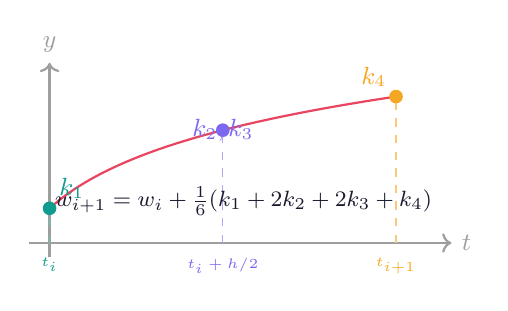
\begin{tikzpicture}[scale=0.88]
			\draw[->,thick,textgray](-0.3,0)--(5.8,0)node[right]{\small$t$};
			\draw[->,thick,textgray](0,-0.2)--(0,2.6)node[above]{\small$y$};
			% curva exacta
			\draw[accent,thick,smooth,domain=0:5,samples=60]
			plot({\x},{0.5+0.9*ln(1+\x)});
			% puntos de evaluación
			\foreach \x/\col/\lab in
			{0/accentteal/{$t_i$},
				2.5/accentviolet/{$t_i+h/2$},
				5/accentamber/{$t_{i+1}$}}{
				\pgfmathsetmacro\yv{0.5+0.9*ln(1+\x)}
				\draw[dashed,\col!60,thin](\x,0)--(\x,\yv);
				\fill[\col](\x,\yv)circle(2.8pt);
				\node[below=2pt,font=\tiny,text=\col]at(\x,0){\lab};
			}
			% etiquetas k1..k4
			\node[above right,font=\small\color{accentteal}]   at (0,{0.5+0.9*ln(1)})     {$k_1$};
			\node[above,font=\small\color{accentviolet}]        at (2.5,{0.5+0.9*ln(2.5)}) {$k_2,k_3$};
			\node[above left,font=\small\color{accentamber}]    at (5,{0.5+0.9*ln(6)})     {$k_4$};
			% pesos
			\node[font=\footnotesize\color{darkbg}]at(2.8,0.6)
			{$w_{i+1}=w_i+\tfrac{1}{6}(k_1+2k_2+2k_3+k_4)$};
		\end{tikzpicture}
	\end{center}
	
	\vspace{2pt}
	\textcolor{textgray}{\small
		Los pesos $1,2,2,1$ corresponden a la cuadratura de Simpson aplicada sobre el intervalo $[t_i,t_{i+1}]$.
		RK4: error local $O(h^5)$, error global $O(h^4)$, cuatro evaluaciones de $f$ por paso.}
\end{frame}

% ─────────────────────────────────────────────────────────
\begin{frame}{Comparaci\'on de la familia de m\'etodos}
	\vspace{6pt}
	\begin{center}
		\renewcommand{\arraystretch}{1.45}
		\begin{tabular}{lccc}
			\toprule
			\textbf{M\'etodo} & \textbf{Evaluaciones} 
			& \textbf{Error global} & \textbf{Cu\'ando usar} \\
			\midrule
			Euler             & 1   & $O(h)$   & prototipo / referencia \\
			Punto medio       & 2   & $O(h^2)$ & problemas simples \\
			Euler modificado  & 2   & $O(h^2)$ & igual que punto medio \\
			Heun (orden 3)    & 3  & $O(h^3)$ & intermedio \\
			\textbf{RK4}      & \textbf{4} &  $O(h^4)$ & \textbf{uso general} \\
			\bottomrule
		\end{tabular}
	\end{center}
	
	\vspace{8pt}
	\begin{obsbox}{Regla pr\'actica}
		Para reducir el error de \textbf{Euler} en $10\times$ hay que reducir $h$ en $10\times$ (10 veces m\'as lento).\\[3pt]
		Para el mismo efecto con \textbf{RK4}: reducir $h$ en $10^{1/4}\approx 1.78\times$.\\[3pt]
		\textcolor{textgray}{\small Con $h=0.1$: error Euler $\sim 10^{-1}$,
			error RK4 $\sim 10^{-4}$.}
	\end{obsbox}
\end{frame}



% ── SECCIÓN: SISTEMA VECTORIAL Y H-K ─────────────────────
\begin{darkslide}
	\begin{frame}[plain]
		\begin{tikzpicture}[remember picture, overlay]
			\fill[coralbox,opacity=0.12]    (current page.north east)++(-2,-2) circle(3.5cm);
			\fill[accentviolet,opacity=0.10](current page.south west)++(1,1)   circle(3cm);
		\end{tikzpicture}
		\vspace{2.5cm}
		\begin{center}
			{\Large\textcolor{textlight}{\textbf{Aplicaci\'on}}}\\[10pt]
			{\large\textcolor{coralbox}{RK4 en sistemas vectoriales}}\\[6pt]
			{\normalsize\textcolor{textgray}{el modelo H-K como PVI de orden 1 en $\R^N$}}
		\end{center}
	\end{frame}
\end{darkslide}

% ─────────────────────────────────────────────────────────
\begin{frame}{Sistema de EDOs de primer orden}
	\vspace{4pt}
	El modelo H-K con $N$ agentes es un \textbf{sistema vectorial}:
	\[
	\frac{du_1}{dt} = f_1(t,u_1,\ldots,u_m),
	\quad \cdots \quad
	\frac{du_m}{dt} = f_m(t,u_1,\ldots,u_m),
	\quad u_j(a) = \alpha_j.
	\]
	En notaci\'on vectorial: $\mathbf{u}'=\mathbf{f}(t,\mathbf{u})$,\;
	$\mathbf{u}(a)=\boldsymbol{\alpha}$.
	
	\vspace{8pt}
	\begin{resultbox}{RK4 vectorial para H-K}
		Los $k_j$ son ahora \textbf{vectores} en $\R^N$:
		\begin{align*}
			\mathbf{k}_1 &= h\,\mathbf{f}(t_i,\;\mathbf{w}_i), \\
			\mathbf{k}_2 &= h\,\mathbf{f}\!\left(t_i+\tfrac{h}{2},\;
			\mathbf{w}_i+\tfrac{1}{2}\mathbf{k}_1\right), \\
			\mathbf{k}_3 &= h\,\mathbf{f}\!\left(t_i+\tfrac{h}{2},\;
			\mathbf{w}_i+\tfrac{1}{2}\mathbf{k}_2\right), \\
			\mathbf{k}_4 &= h\,\mathbf{f}\!\left(t_i+h,\;
			\mathbf{w}_i+\mathbf{k}_3\right), \\
			\mathbf{w}_{i+1} &= \mathbf{w}_i
			+ \tfrac{1}{6}(\mathbf{k}_1+2\mathbf{k}_2+2\mathbf{k}_3+\mathbf{k}_4).
		\end{align*}
		\textcolor{textgray}{\small
			El c\'odigo es id\'entico al escalar: NumPy opera en arrays de cualquier dimensi\'on.}
	\end{resultbox}
\end{frame}

% ─────────────────────────────────────────────────────────
%\begin{frame}[fragile]{Pausa: implementar y comparar}
%	\vspace{2pt}
%	\begin{columns}[T]
%		\column{0.52\textwidth}
%		\begin{lstlisting}
%			def rk4(f, w0, t, **kw):
%			W = np.zeros((len(t), len(w0)))
%			W[0] = w0
%			for i in range(len(t) - 1):
%			h  = t[i+1] - t[i]
%			k1 = h * f(t[i],         W[i],           **kw)
%			k2 = h * f(t[i] + h/2,   W[i] + k1/2,   **kw)
%			k3 = h * f(t[i] + h/2,   W[i] + k2/2,   **kw)
%			k4 = h * f(t[i] + h,     W[i] + k3,      **kw)
%			W[i+1] = W[i] + (k1+2*k2+2*k3+k4)/6
%			return W   # shape (M, N)
%		\end{lstlisting}
%		
%		\vspace{4pt}
%		\textcolor{textgray}{\small
%			Notar que $k_j = h\cdot f(\ldots)$: la $h$ se absorbe
%			en el $k$, igual que en la definici\'on.}
%		
%		\column{0.45\textwidth}
%		\begin{taskbox}{Ejercicio en notebook}
%			Con $N=30$, $\varepsilon=0.45$ y $h\in\{0.5,\,0.1,\,0.01\}$:\\[4pt]
%			\textbf{(a)} Comparar las trayectorias de Euler y RK4.\\[3pt]
%			\textbf{(b)} Graficar el error vs.\ la soluci\'on de referencia
%			(RK4 con $h=10^{-4}$) en escala log-log.\\[3pt]
%			\textbf{(c)} Medir la pendiente de la curva de error: ?`confirma $O(h)$ para Euler y $O(h^4)$ para RK4?
%		\end{taskbox}
%	\end{columns}
%\end{frame}

% ── CIERRE ────────────────────────────────────────────────
%\begin{darkslide}
%	\begin{frame}[plain]
%		\begin{tikzpicture}[remember picture, overlay]
%			\fill[accent,opacity=0.15]      (current page.north east)++(-1,-1)   circle(3.5cm);
%			\fill[accentteal,opacity=0.10]  (current page.south west)++(2,2)     circle(2.8cm);
%			\fill[accentviolet,opacity=0.08](current page.north west)++(1,-2)    circle(2cm);
%		\end{tikzpicture}
%		\vspace{1.8cm}
%		\begin{center}
%			{\large\textcolor{textgray}{Recapitulando}}\\[12pt]
%			{\large\textcolor{textlight}{\textbf{Euler}}}\\
%			{\small\textcolor{textgray}{$w_{i+1}=w_i+h f(t_i,w_i)$\;---\;
%					error global $O(h)$,\; 1 evaluaci\'on}}\\[8pt]
%			{\large\textcolor{textlight}{\textbf{Taylor de orden $n$}}}\\
%			{\small\textcolor{textgray}{precisci\'on $O(h^n)$ pero requiere derivar $f$
%					--- no es factible en general}}\\[8pt]
%			{\large\textcolor{textlight}{\textbf{RK4}}}\\
%			{\small\textcolor{textgray}{$w_{i+1}=w_i+\tfrac{1}{6}(k_1+2k_2+2k_3+k_4)$\;---\;
%					error $O(h^4)$,\; 4 evaluaciones}}\\[8pt]
%			{\large\textcolor{textlight}{\textbf{Tripleta de oro}}}\\
%			{\small\textcolor{textgray}{consistencia + Lipschitz $\Rightarrow$ convergencia y estabilidad}}\\[14pt]
%			\rule{4cm}{0.4pt}\\[6pt]
%			{\small\textcolor{textgray}{\texttt{mbastidaso@unal.edu.co}}}
%		\end{center}
%	\end{frame}
%\end{darkslide}


\end{document}
